\documentclass[NET,english,beameralt]{tumbeamer}

\usepackage{listings}
\documentclass[NET,english,beameralt]{tumbeamer}
\usepackage[options]{minted}
\usepackage[options]{hyperref}
\documentclass[NET,english,beameralt]{tumbeamer}
\usepackage[options]{minted}
\usepackage[options]{hyperref}
\documentclass[NET,english,beameralt]{tumbeamer}
\usepackage[options]{minted}
\usepackage[options]{hyperref}
\input{include/slides}
\beamerdefaultoverlayspecification{<+->}

\begin{document}

\begin{frame}{Agenda}
    \begin{itemize}[<.->]
        \item Starlink 101
        \item trying to understand routing decisions
        \item visualize visible satellites
        \item exploring the GRPC api
    \end{itemize}
\end{frame}

\begin{frame}{Starlink 101}
\begin{figure}
    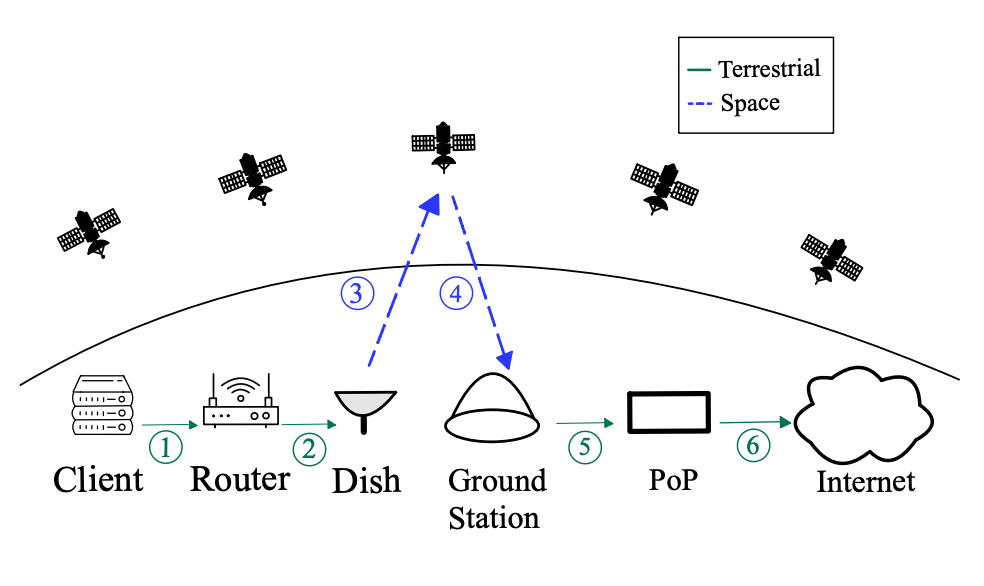
\includegraphics[width=0.75\textwidth]{pics/starlink-101.png}
    \caption[short]{Basic Starlink working (ignoring ISL), from \cite{izhikevich2023democratizing}}
\end{figure}
\end{frame}

\begin{frame}{Understanding routing decisions}
\begin{itemize}
    \item got ip address blocks from major cloud providers (aws,azure,oracle), as we know their position \footnote[]{the fact we know the position doesn't really mean a traceroute to a certain address is really a traceroute to that geographic area}
    \item chose 5 geographically sparse targets around the globe (for aws: ap-northeast-2, us-east-1, ap-south-1, sa-east-1, me-south-1 )
    \item tracerouted the targets over several days 
\end{itemize}
\end{frame}

\begin{frame}{Understanding routing decisions}
\begin{figure}
    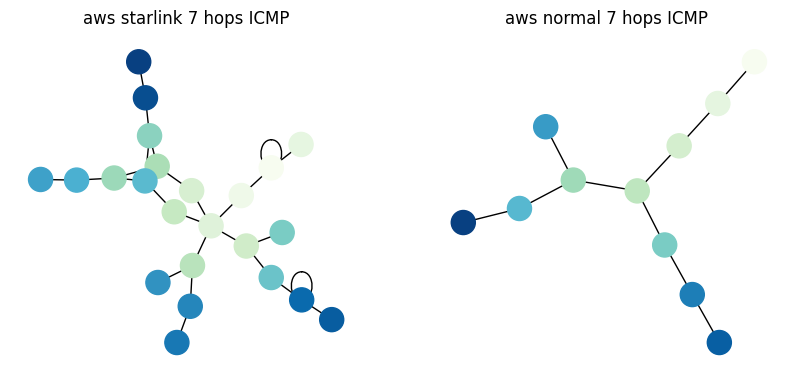
\includegraphics[width=0.75\textwidth]{pics/aws_7_icmp.png}
    \caption[short]{First 7 hops of traceroutes to 5 AWS datacenters using ICMP}
\end{figure}
\end{frame}

\begin{frame}{Understanding routing decisions}
\begin{figure}
    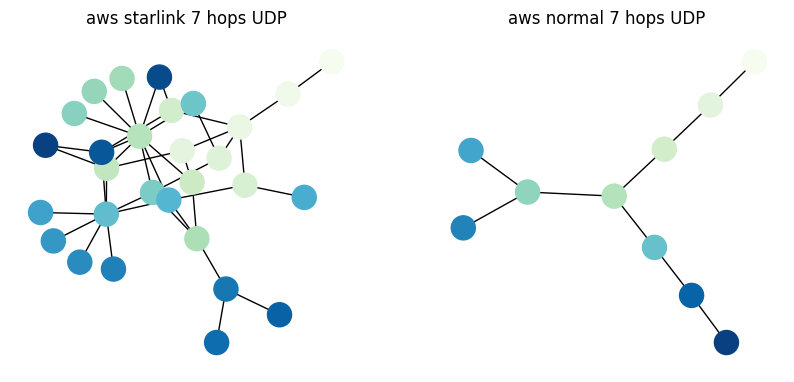
\includegraphics[width=0.75\textwidth]{pics/aws_7_udp.png}
    \caption[short]{First 7 hops of traceroutes to 5 AWS datacenters using UDP}
\end{figure}
\end{frame}

\begin{frame}{Understanding routing decisions}
\begin{figure}
    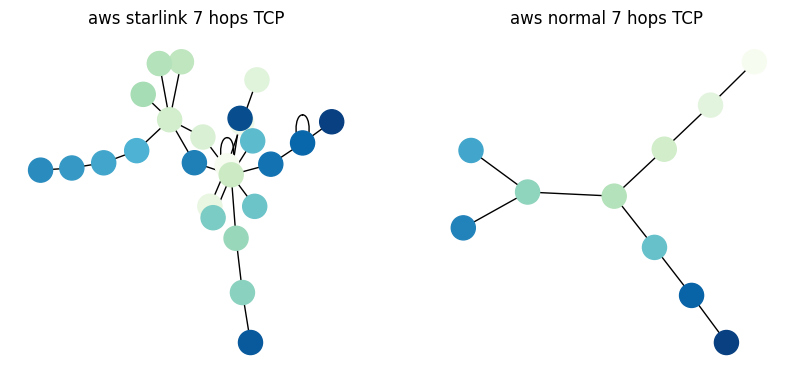
\includegraphics[width=0.75\textwidth]{pics/aws_7_tcp.png}
    \caption[short]{First 7 hops of traceroutes to 5 AWS datacenters using TCP}
\end{figure}
\end{frame}

\begin{frame}{measuring RTT changes when applying stress iperf}
\begin{figure}
    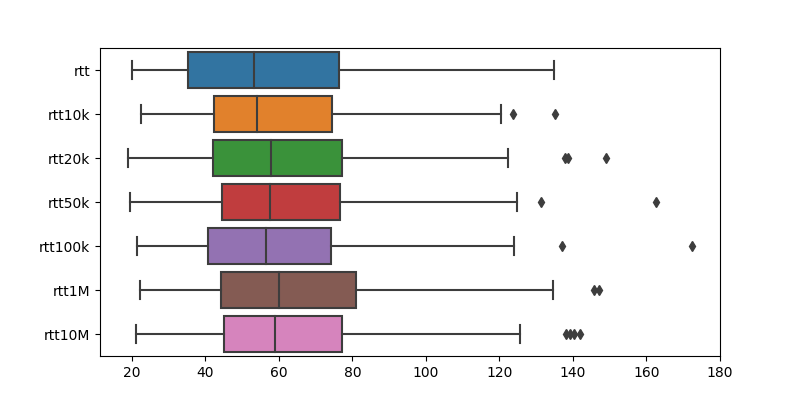
\includegraphics[width=1\textwidth]{pics/rtt-iperf-stress.png}
    \caption[short]{measuring RTT changes when applying stress iperf}
\end{figure}
\end{frame}

\begin{frame}{Visualize visible satellites}
\begin{itemize}
    \item from \href{celestrak.org}{celestrak.org} we can download a list of Starlink's satellites TLEs
    \item A two-line element set (TLE) is a data format encoding a list of orbital elements of an Earth-orbiting object for a given point in time, the epoch. Using a suitable prediction formula, the state (position and velocity) at any point in the past or future can be estimated to some accuracy. (from wikipedia.org)
\end{itemize}
\end{frame}

\begin{frame}[fragile]{\texttt{common.calculate\_visible\_satellites}}
\begin{minted}[fontsize=\small]{python3}
def calculate_visible_satellites(...):
    # ...
    satellites = load.tle_file(stations_url)
    observer = Topos(observer_latitude, observer_longitude, observer_elevation)
    t = load.timescale().now()

    # Calculate satellite positions
    positions = [(sat, (sat - observer).at(t)) for sat in satellites]
    
    # Filter visible satellites
    visible_satellites = []
    for sat, position in positions:
        alt, az, distance = position.altaz()
        # Satellite is above the horizon
        if alt.degrees > 0 and distance.km < distance_km:
            visible_satellites.append((sat, alt, az))

    return visible_satellites
\end{minted}
\end{frame}

\begin{frame}{count of visible satellites across time}
\begin{figure}
    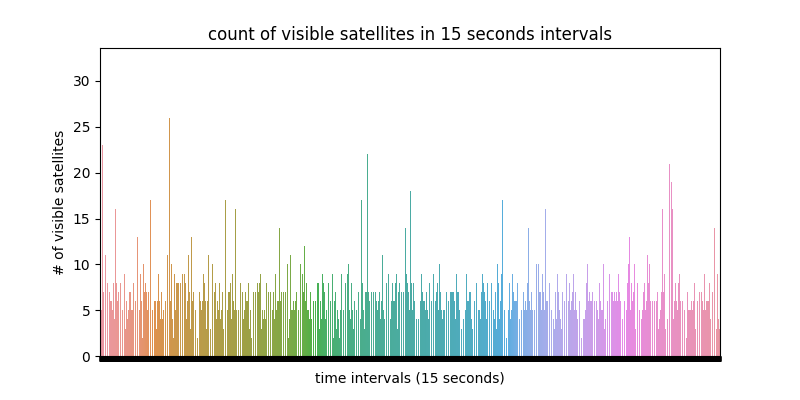
\includegraphics[width=1\textwidth]{pics/count_visible_satellites.png}
    \caption[short]{count of visible satellites across time}
\end{figure}
\end{frame}

\begin{frame}{visualizing patterns in visible satellites}
\begin{figure}
    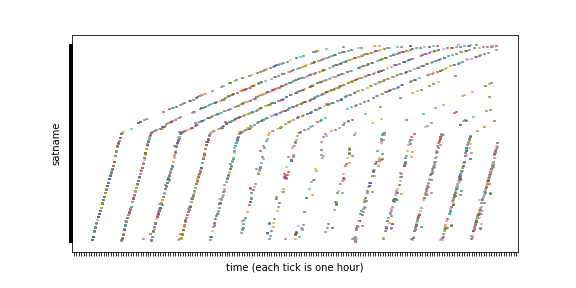
\includegraphics[width=1\textwidth]{pics/visualizing-how-long-satellites-are-visible-for.png}
    \caption[short]{visualizing patterns in visible satellites}
\end{figure}
\end{frame}

\begin{frame}{the gRPC api}
\begin{itemize}
    \item the dish exposes a gRPC api with server reflection, "runtime construction of requests without having stub information precompiled into the client." \footnote{\href{https://github.com/grpc/grpc/blob/master/doc/server-reflection.md}{https://github.com/grpc/grpc/blob/master/doc/server-reflection.md}}
    \item 55 "methods" are available, most of them don't work, we have 2 categories of errors: \texttt{Uninmplemented}, \texttt{PermissionDenied} and a couple of some other specific errors 
    \item working methods: \texttt{reboot}, \texttt{get\_status}, \texttt{start\_dish\_self\_test}, \texttt{get\_history}, \texttt{get\_device\_info}, \texttt{dish\_power\_save}, \texttt{dish\_get\_config}, \texttt{get\_obstruction\_map}
    \item to see all methods: \href{https://hedgedoc.net.in.tum.de/N7nACD1OSk2x2e7biPHJTA}{https://hedgedoc.net.in.tum.de/N7nACD1OSk2x2e7biPHJTA}
\end{itemize}
\end{frame}

\begin{frame}{next actions}
\begin{itemize}
    \item investigate satellite handovers following the method described in \cite{izhikevich2023democratizing} (we have a script working)
    \item try to correlate satellite handovers with sudden drops in bandwidth
    \item sneak peak: \href{https://youtu.be/PjfMPr20suw}{https://youtu.be/PjfMPr20suw}
\end{itemize}
\end{frame}

\section{Bibliography}
\begin{frame}[allowframebreaks]
    \bibliographystyle{abbrv}
    \setbeamertemplate{bibliography item}[text]
    \footnotesize
    \bibliography{lit}
\end{frame}

\end{document}

\beamerdefaultoverlayspecification{<+->}

\begin{document}

\begin{frame}{Agenda}
    \begin{itemize}[<.->]
        \item Starlink 101
        \item trying to understand routing decisions
        \item visualize visible satellites
        \item exploring the GRPC api
    \end{itemize}
\end{frame}

\begin{frame}{Starlink 101}
\begin{figure}
    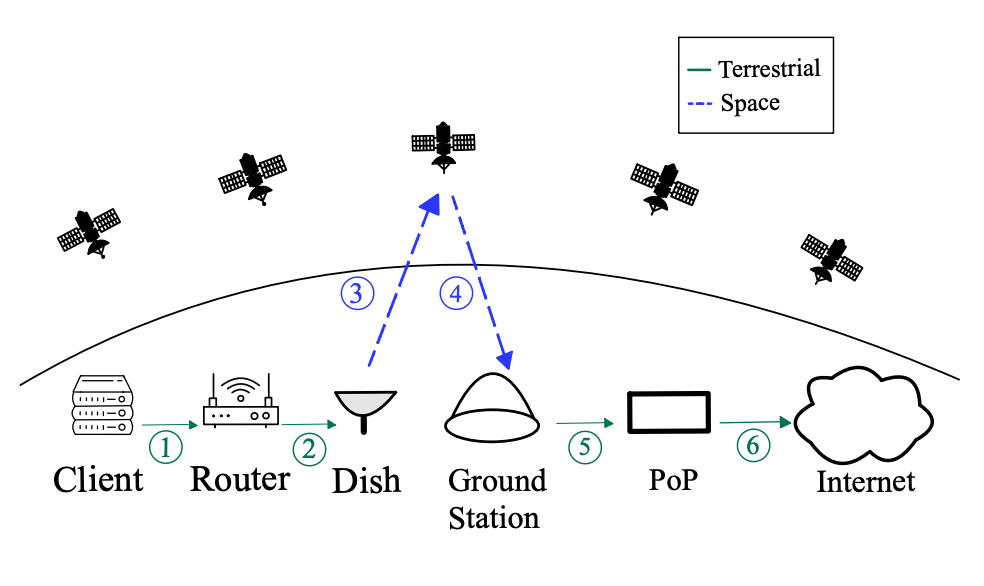
\includegraphics[width=0.75\textwidth]{pics/starlink-101.png}
    \caption[short]{Basic Starlink working (ignoring ISL), from \cite{izhikevich2023democratizing}}
\end{figure}
\end{frame}

\begin{frame}{Understanding routing decisions}
\begin{itemize}
    \item got ip address blocks from major cloud providers (aws,azure,oracle), as we know their position \footnote[]{the fact we know the position doesn't really mean a traceroute to a certain address is really a traceroute to that geographic area}
    \item chose 5 geographically sparse targets around the globe (for aws: ap-northeast-2, us-east-1, ap-south-1, sa-east-1, me-south-1 )
    \item tracerouted the targets over several days 
\end{itemize}
\end{frame}

\begin{frame}{Understanding routing decisions}
\begin{figure}
    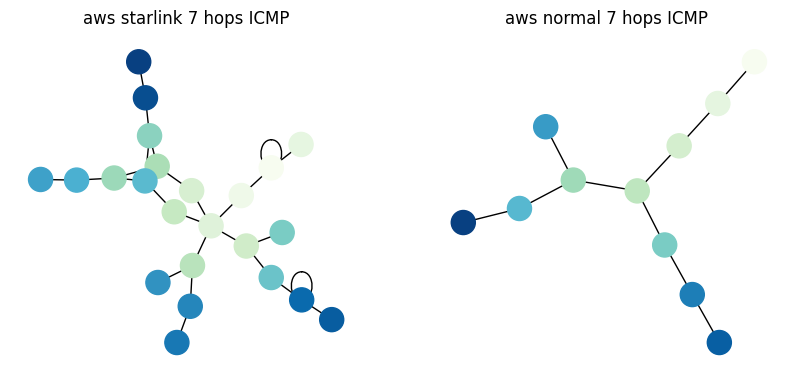
\includegraphics[width=0.75\textwidth]{pics/aws_7_icmp.png}
    \caption[short]{First 7 hops of traceroutes to 5 AWS datacenters using ICMP}
\end{figure}
\end{frame}

\begin{frame}{Understanding routing decisions}
\begin{figure}
    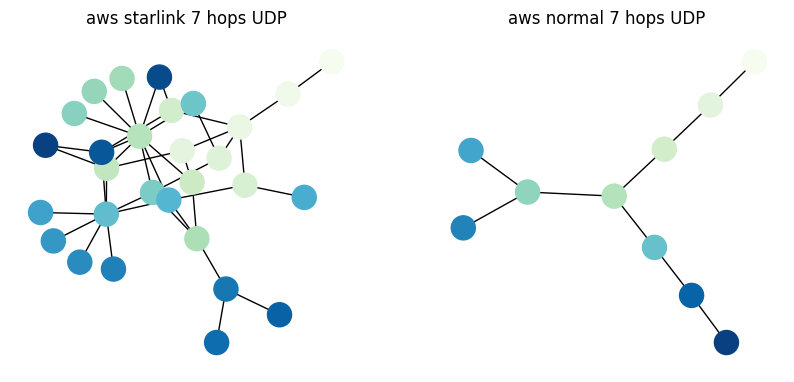
\includegraphics[width=0.75\textwidth]{pics/aws_7_udp.png}
    \caption[short]{First 7 hops of traceroutes to 5 AWS datacenters using UDP}
\end{figure}
\end{frame}

\begin{frame}{Understanding routing decisions}
\begin{figure}
    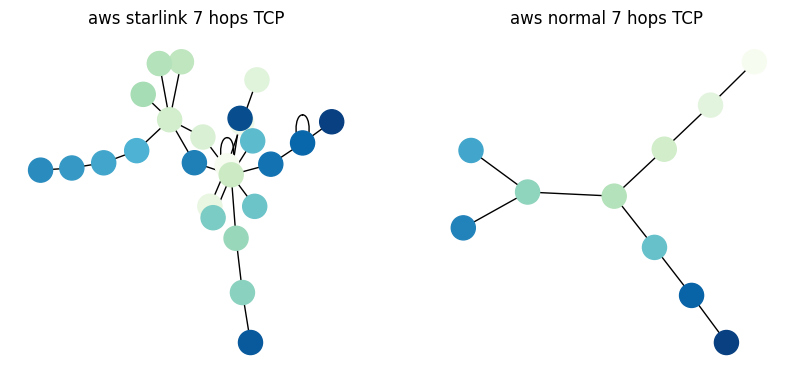
\includegraphics[width=0.75\textwidth]{pics/aws_7_tcp.png}
    \caption[short]{First 7 hops of traceroutes to 5 AWS datacenters using TCP}
\end{figure}
\end{frame}

\begin{frame}{measuring RTT changes when applying stress iperf}
\begin{figure}
    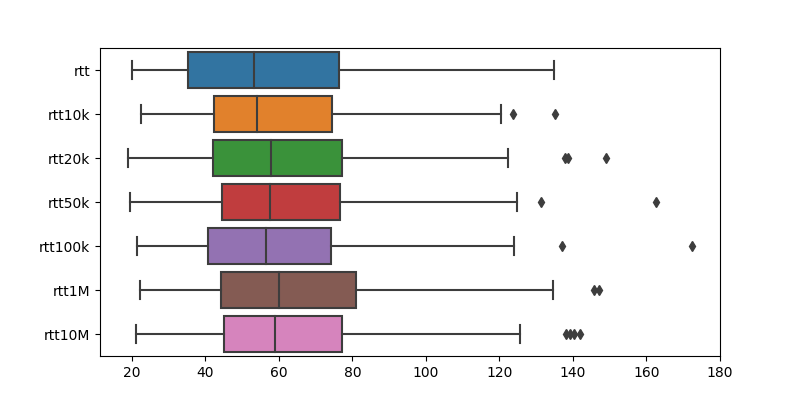
\includegraphics[width=1\textwidth]{pics/rtt-iperf-stress.png}
    \caption[short]{measuring RTT changes when applying stress iperf}
\end{figure}
\end{frame}

\begin{frame}{Visualize visible satellites}
\begin{itemize}
    \item from \href{celestrak.org}{celestrak.org} we can download a list of Starlink's satellites TLEs
    \item A two-line element set (TLE) is a data format encoding a list of orbital elements of an Earth-orbiting object for a given point in time, the epoch. Using a suitable prediction formula, the state (position and velocity) at any point in the past or future can be estimated to some accuracy. (from wikipedia.org)
\end{itemize}
\end{frame}

\begin{frame}[fragile]{\texttt{common.calculate\_visible\_satellites}}
\begin{minted}[fontsize=\small]{python3}
def calculate_visible_satellites(...):
    # ...
    satellites = load.tle_file(stations_url)
    observer = Topos(observer_latitude, observer_longitude, observer_elevation)
    t = load.timescale().now()

    # Calculate satellite positions
    positions = [(sat, (sat - observer).at(t)) for sat in satellites]
    
    # Filter visible satellites
    visible_satellites = []
    for sat, position in positions:
        alt, az, distance = position.altaz()
        # Satellite is above the horizon
        if alt.degrees > 0 and distance.km < distance_km:
            visible_satellites.append((sat, alt, az))

    return visible_satellites
\end{minted}
\end{frame}

\begin{frame}{count of visible satellites across time}
\begin{figure}
    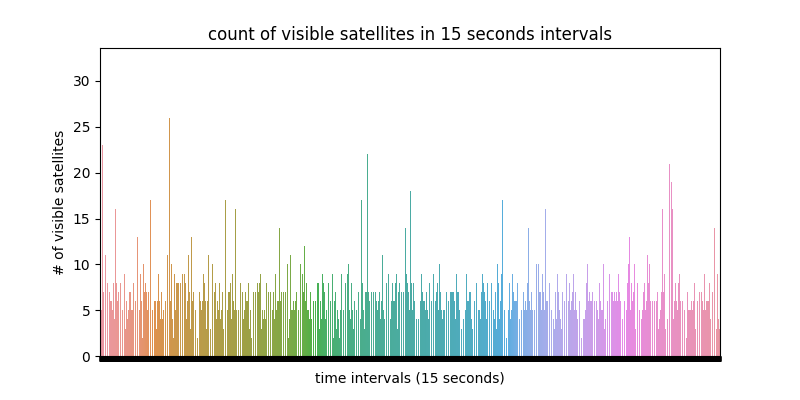
\includegraphics[width=1\textwidth]{pics/count_visible_satellites.png}
    \caption[short]{count of visible satellites across time}
\end{figure}
\end{frame}

\begin{frame}{visualizing patterns in visible satellites}
\begin{figure}
    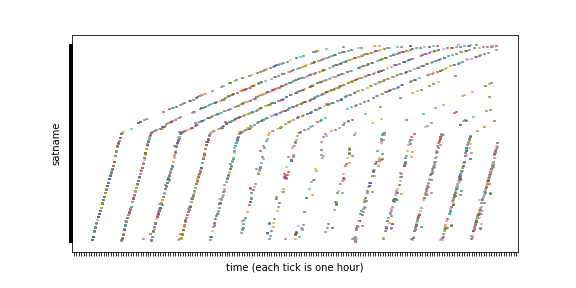
\includegraphics[width=1\textwidth]{pics/visualizing-how-long-satellites-are-visible-for.png}
    \caption[short]{visualizing patterns in visible satellites}
\end{figure}
\end{frame}

\begin{frame}{the gRPC api}
\begin{itemize}
    \item the dish exposes a gRPC api with server reflection, "runtime construction of requests without having stub information precompiled into the client." \footnote{\href{https://github.com/grpc/grpc/blob/master/doc/server-reflection.md}{https://github.com/grpc/grpc/blob/master/doc/server-reflection.md}}
    \item 55 "methods" are available, most of them don't work, we have 2 categories of errors: \texttt{Uninmplemented}, \texttt{PermissionDenied} and a couple of some other specific errors 
    \item working methods: \texttt{reboot}, \texttt{get\_status}, \texttt{start\_dish\_self\_test}, \texttt{get\_history}, \texttt{get\_device\_info}, \texttt{dish\_power\_save}, \texttt{dish\_get\_config}, \texttt{get\_obstruction\_map}
    \item to see all methods: \href{https://hedgedoc.net.in.tum.de/N7nACD1OSk2x2e7biPHJTA}{https://hedgedoc.net.in.tum.de/N7nACD1OSk2x2e7biPHJTA}
\end{itemize}
\end{frame}

\begin{frame}{next actions}
\begin{itemize}
    \item investigate satellite handovers following the method described in \cite{izhikevich2023democratizing} (we have a script working)
    \item try to correlate satellite handovers with sudden drops in bandwidth
    \item sneak peak: \href{https://youtu.be/PjfMPr20suw}{https://youtu.be/PjfMPr20suw}
\end{itemize}
\end{frame}

\section{Bibliography}
\begin{frame}[allowframebreaks]
    \bibliographystyle{abbrv}
    \setbeamertemplate{bibliography item}[text]
    \footnotesize
    \bibliography{lit}
\end{frame}

\end{document}

\beamerdefaultoverlayspecification{<+->}

\begin{document}

\begin{frame}{Agenda}
    \begin{itemize}[<.->]
        \item Starlink 101
        \item trying to understand routing decisions
        \item visualize visible satellites
        \item exploring the GRPC api
    \end{itemize}
\end{frame}

\begin{frame}{Starlink 101}
\begin{figure}
    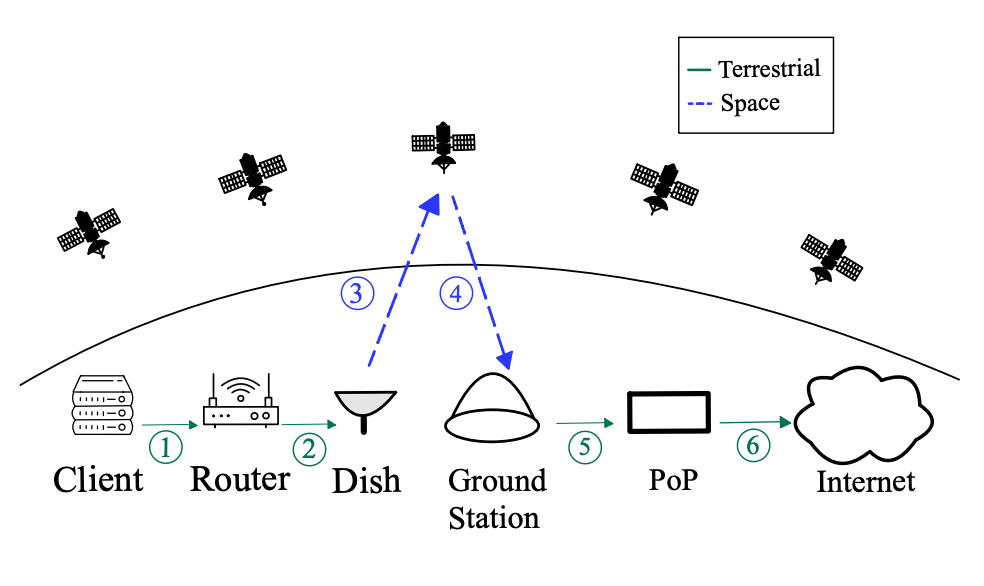
\includegraphics[width=0.75\textwidth]{pics/starlink-101.png}
    \caption[short]{Basic Starlink working (ignoring ISL), from \cite{izhikevich2023democratizing}}
\end{figure}
\end{frame}

\begin{frame}{Understanding routing decisions}
\begin{itemize}
    \item got ip address blocks from major cloud providers (aws,azure,oracle), as we know their position \footnote[]{the fact we know the position doesn't really mean a traceroute to a certain address is really a traceroute to that geographic area}
    \item chose 5 geographically sparse targets around the globe (for aws: ap-northeast-2, us-east-1, ap-south-1, sa-east-1, me-south-1 )
    \item tracerouted the targets over several days 
\end{itemize}
\end{frame}

\begin{frame}{Understanding routing decisions}
\begin{figure}
    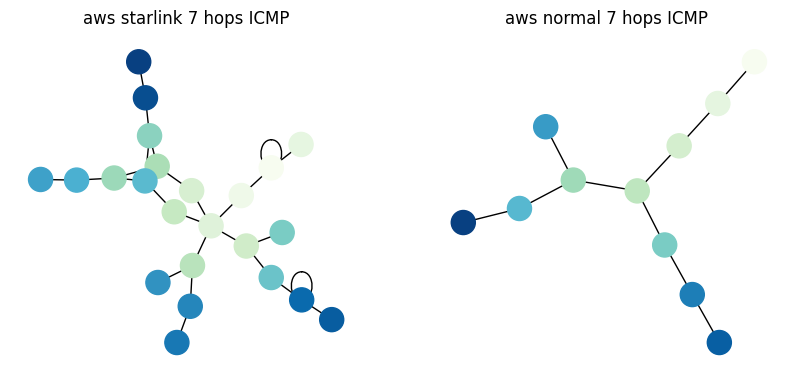
\includegraphics[width=0.75\textwidth]{pics/aws_7_icmp.png}
    \caption[short]{First 7 hops of traceroutes to 5 AWS datacenters using ICMP}
\end{figure}
\end{frame}

\begin{frame}{Understanding routing decisions}
\begin{figure}
    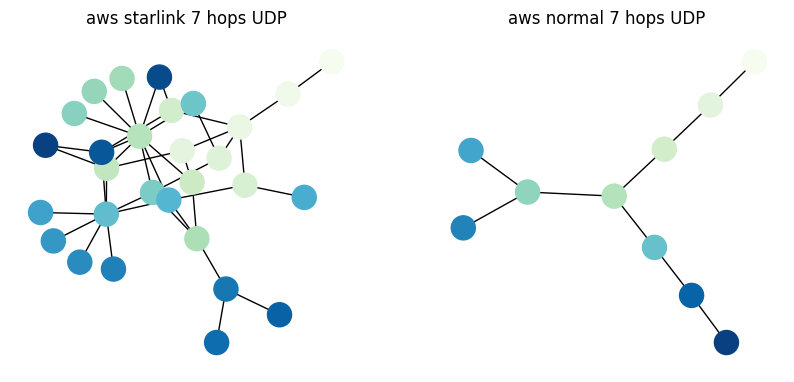
\includegraphics[width=0.75\textwidth]{pics/aws_7_udp.png}
    \caption[short]{First 7 hops of traceroutes to 5 AWS datacenters using UDP}
\end{figure}
\end{frame}

\begin{frame}{Understanding routing decisions}
\begin{figure}
    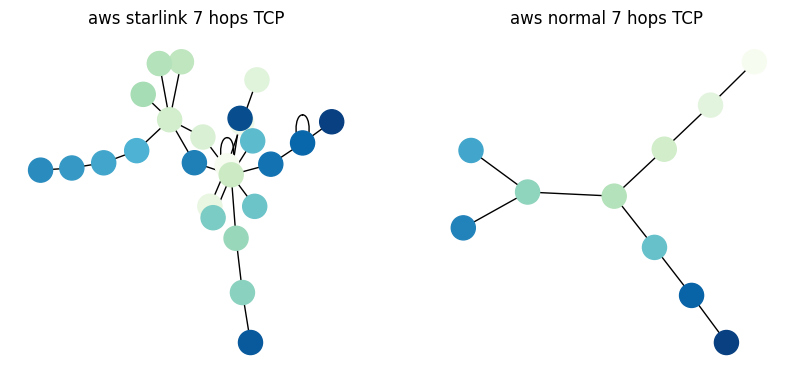
\includegraphics[width=0.75\textwidth]{pics/aws_7_tcp.png}
    \caption[short]{First 7 hops of traceroutes to 5 AWS datacenters using TCP}
\end{figure}
\end{frame}

\begin{frame}{measuring RTT changes when applying stress iperf}
\begin{figure}
    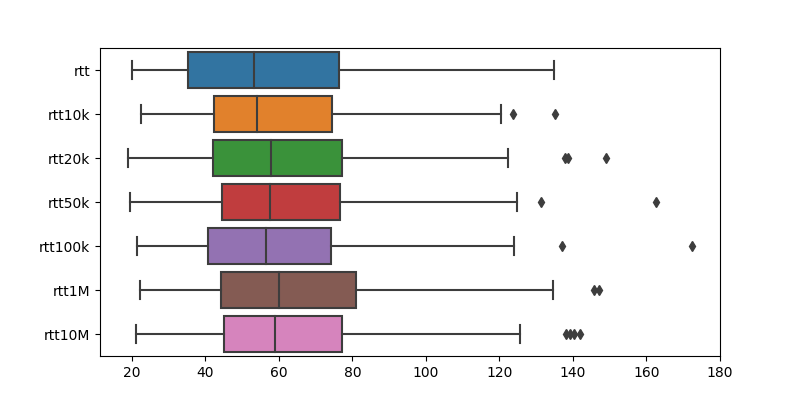
\includegraphics[width=1\textwidth]{pics/rtt-iperf-stress.png}
    \caption[short]{measuring RTT changes when applying stress iperf}
\end{figure}
\end{frame}

\begin{frame}{Visualize visible satellites}
\begin{itemize}
    \item from \href{celestrak.org}{celestrak.org} we can download a list of Starlink's satellites TLEs
    \item A two-line element set (TLE) is a data format encoding a list of orbital elements of an Earth-orbiting object for a given point in time, the epoch. Using a suitable prediction formula, the state (position and velocity) at any point in the past or future can be estimated to some accuracy. (from wikipedia.org)
\end{itemize}
\end{frame}

\begin{frame}[fragile]{\texttt{common.calculate\_visible\_satellites}}
\begin{minted}[fontsize=\small]{python3}
def calculate_visible_satellites(...):
    # ...
    satellites = load.tle_file(stations_url)
    observer = Topos(observer_latitude, observer_longitude, observer_elevation)
    t = load.timescale().now()

    # Calculate satellite positions
    positions = [(sat, (sat - observer).at(t)) for sat in satellites]
    
    # Filter visible satellites
    visible_satellites = []
    for sat, position in positions:
        alt, az, distance = position.altaz()
        # Satellite is above the horizon
        if alt.degrees > 0 and distance.km < distance_km:
            visible_satellites.append((sat, alt, az))

    return visible_satellites
\end{minted}
\end{frame}

\begin{frame}{count of visible satellites across time}
\begin{figure}
    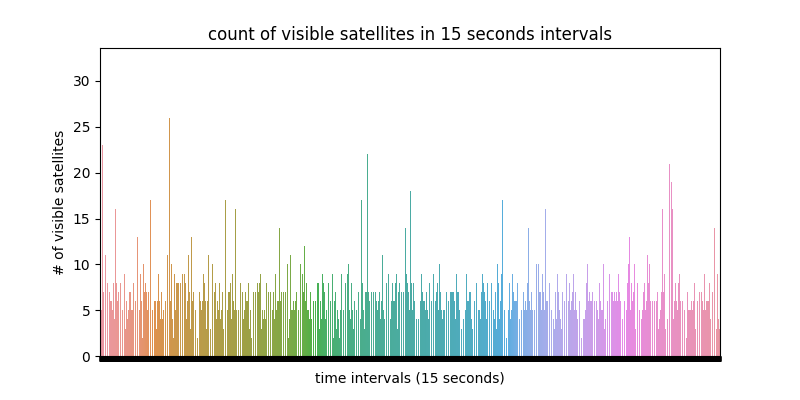
\includegraphics[width=1\textwidth]{pics/count_visible_satellites.png}
    \caption[short]{count of visible satellites across time}
\end{figure}
\end{frame}

\begin{frame}{visualizing patterns in visible satellites}
\begin{figure}
    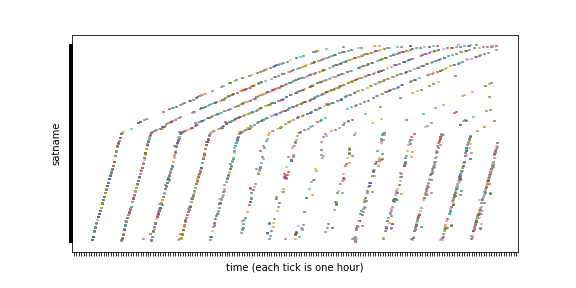
\includegraphics[width=1\textwidth]{pics/visualizing-how-long-satellites-are-visible-for.png}
    \caption[short]{visualizing patterns in visible satellites}
\end{figure}
\end{frame}

\begin{frame}{the gRPC api}
\begin{itemize}
    \item the dish exposes a gRPC api with server reflection, "runtime construction of requests without having stub information precompiled into the client." \footnote{\href{https://github.com/grpc/grpc/blob/master/doc/server-reflection.md}{https://github.com/grpc/grpc/blob/master/doc/server-reflection.md}}
    \item 55 "methods" are available, most of them don't work, we have 2 categories of errors: \texttt{Uninmplemented}, \texttt{PermissionDenied} and a couple of some other specific errors 
    \item working methods: \texttt{reboot}, \texttt{get\_status}, \texttt{start\_dish\_self\_test}, \texttt{get\_history}, \texttt{get\_device\_info}, \texttt{dish\_power\_save}, \texttt{dish\_get\_config}, \texttt{get\_obstruction\_map}
    \item to see all methods: \href{https://hedgedoc.net.in.tum.de/N7nACD1OSk2x2e7biPHJTA}{https://hedgedoc.net.in.tum.de/N7nACD1OSk2x2e7biPHJTA}
\end{itemize}
\end{frame}

\begin{frame}{next actions}
\begin{itemize}
    \item investigate satellite handovers following the method described in \cite{izhikevich2023democratizing} (we have a script working)
    \item try to correlate satellite handovers with sudden drops in bandwidth
    \item sneak peak: \href{https://youtu.be/PjfMPr20suw}{https://youtu.be/PjfMPr20suw}
\end{itemize}
\end{frame}

\section{Bibliography}
\begin{frame}[allowframebreaks]
    \bibliographystyle{abbrv}
    \setbeamertemplate{bibliography item}[text]
    \footnotesize
    \bibliography{lit}
\end{frame}

\end{document}


\begin{document}

\begin{frame}{What is Starlink?}
    \begin{itemize}
        \item Starlink is a Low Earth Orbiting (LEO) satellite constellation
        \item 4000+ satellites with plans to launch more
        \item End users have a Dish to connect to satellites in sight
        \item Performance is higher compared to geostationary satellites (GEOSAT) based connections (\textasciitilde 550
              km in height vs \textasciitilde 35,000 km)
        \item Average latency is ~35 ms, download bandwidth is $>$ 100 MBps
    \end{itemize}

    \begin{figure}
        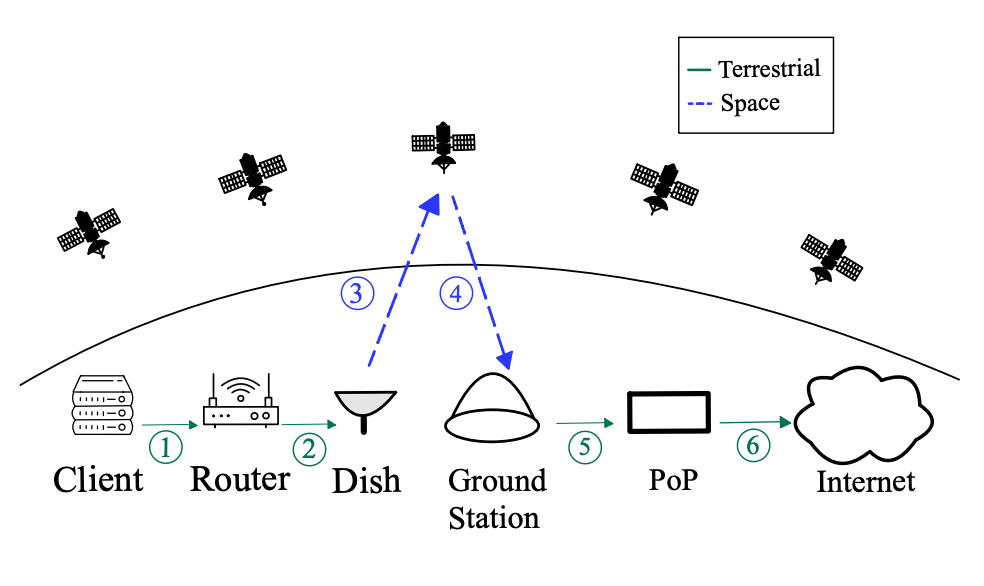
\includegraphics[width=0.45\textwidth]{pics/starlink-101.png}
        \caption{Starlink in a nutshell (ignoring Inter Satellite Links), from \cite{izhikevich2023democratizing}}
    \end{figure}
\end{frame}

\begin{frame}{Our Dish}
    \begin{figure}
        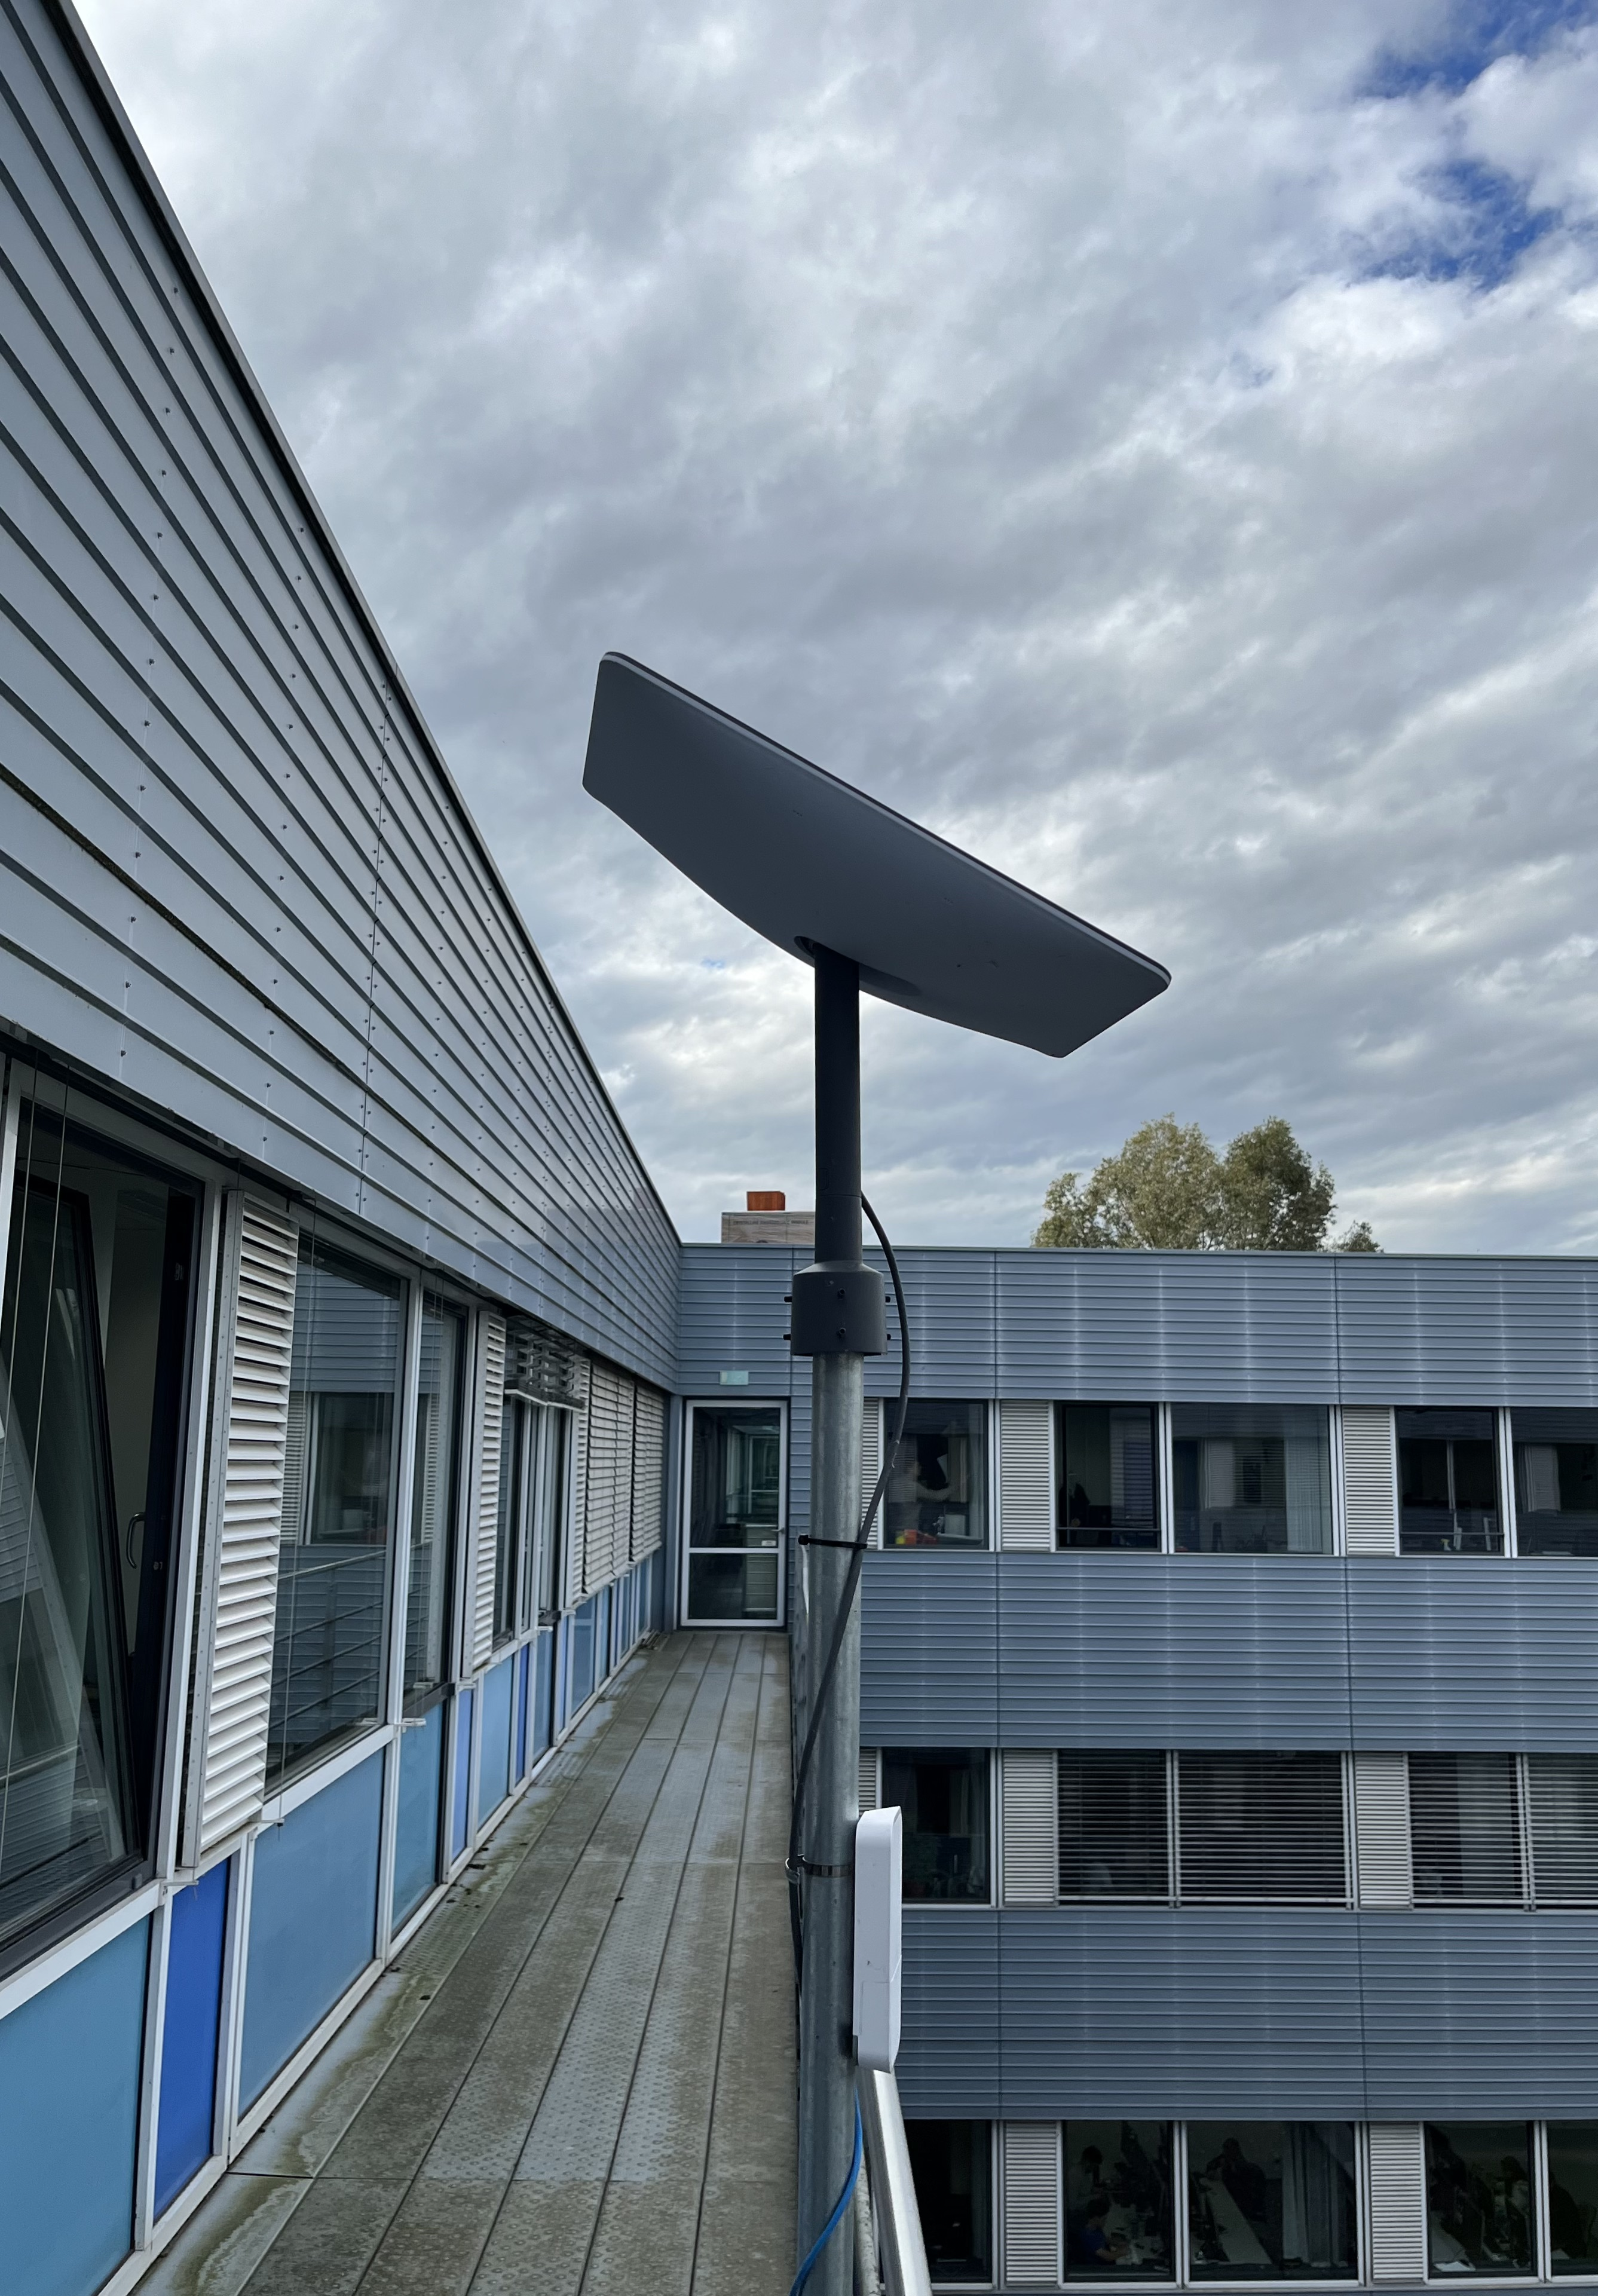
\includegraphics[width=0.3\textwidth]{pics/dish.jpeg}
    \end{figure}
\end{frame}

\begin{frame}{Problem Statement}
    \begin{itemize}
        \item Documenting gRPC API
        \item Can we measure latency to the Point of Presence (PoP)?
        \item Can we gather additional information about routing inside AS14593 
              \footnote{The Autonomous System SpaceX opearates; \url{https://www.peeringdb.com/net/18747}}?
        \item Can we visualize visible satellites?
        \item Is there any correlation between satellite handovers and drops in bandwidth?
            \begin{itemize}
                \item Retrieval of obstruction maps
                \item Satellite handovers detection based on obstruction maps
            \end{itemize}
    \end{itemize}
\end{frame}

\begin{frame}{Similar Technologies}
    \begin{itemize}
        \item Eutelsat operates a LEO constellation, Oneweb \footnote{\url{https://oneweb.net}}, mainly serving
              Enterprises and Governments
        \item Amazon is currently launching its own LEO constellation: Project Kuiper
              \footnote{https://www.aboutamazon.com/what-we-do/devices-services/project-kuiper}, with plans to launch
              3,236 satellites, with secured lanches (BlueOrigin)
        \item The China Aerospace Science and Technology Corporation plans to deploy a 13,000-satellite constellation
              \footnote{\url{https://spacenews.com/china-to-begin-constructing-its-own-megaconstellation-later-this-year/}}
        \item The increasing number of LEO satellites might cause problems, mainly:
        \begin{itemize}
            \item Overall sky brightness increases (impacts astronomical observation)
            \item Proliferation of debris
        \end{itemize}
        \item It is important to work on tooling to better understand the infrastructure
    \end{itemize}
\end{frame}

\begin{frame}{Documenting the gRPC API}
    \begin{itemize}
        \item We started by documenting the gRPC\footnote{\url{https://grpc.io} is a RPC framework from Google} API
              running on the dish
        \item API is reachable at \texttt{192.168.100.1:9200}
        \item The dish exposes a gRPC API with \emph{"Server Reflection"}\footnote{"Runtime construction of requests
              without having stub information precompiled into the client."
              \url{https://github.com/grpc/grpc/blob/master/doc/server-reflection.md}}
        \item 55 endpoints are available
        \begin{itemize}
            \item Majority of them do not work
            \item 2 categories of errors: \texttt{Uninmplemented}, \texttt{PermissionDenied} and a some other errors 
        \end{itemize}
        \item Most interesting working endpoints
              \footnote{\url{https://gist.github.com/rcastellotti/e20630366dfeaeada6cc2680f562f6ac}}: 
            \begin{itemize}
                \item \texttt{reboot}
                \item \texttt{get\_status}
                \item \texttt{get\_obstruction\_map}
            \end{itemize}
    \end{itemize}
\end{frame}

\begin{frame}{Measuring Latency to the Point of Presence}
    Can we measure latency to the Point of Presence (PoP)?
    \begin{itemize}
        \item In short, we don't have to
        \item The \texttt{get\_status} endpoint contains a  \texttt{pop\_ping\_latency\_ms} field
        \item We started polling the endpoint to gather latency to the Point of Presence
        \pause
        \item Latency is pretty stable, averaging ~35 ms with some irregular peaks
        \item Data reported by the API seems to be consistent with traceroutes
    \end{itemize}
    \begin{figure}
        \centering
        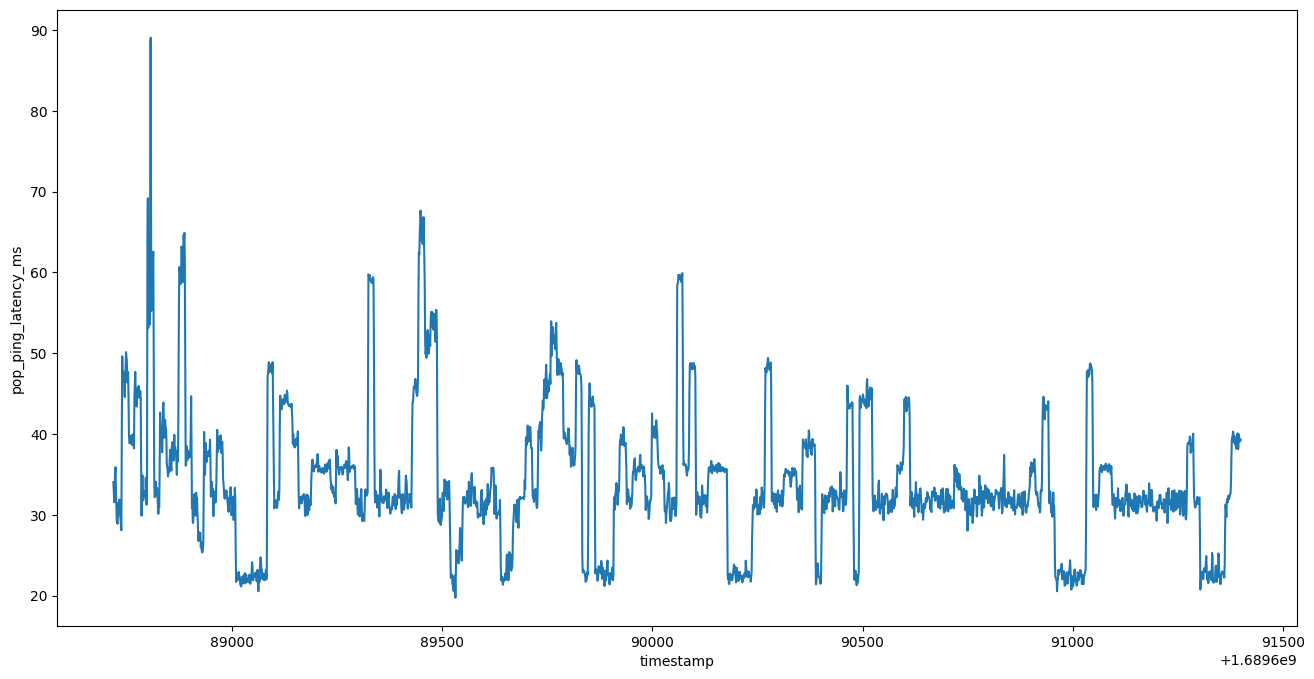
\includegraphics[width=0.6\columnwidth]{pics/latency.png}
    \end{figure}
\end{frame}

\begin{frame}{Understanding Routing Decisions}
    Can we gather additional information about routing inside AS14593 
        \footnote{The Autonomous System SpaceX opearates; \url{https://www.peeringdb.com/net/18747}}?
    \begin{itemize}
        \item Retrieved IP address blocks from major cloud providers (AWS, Azure, Oracle), position already known
            \footnote{does not necessarily mean the last hop will be in that area (little information around what happens inside data centers), 
                        but a good enough approximation}
        \item Chose five geographically sparse targets around the globe, i.e., for aws:
            \begin{itemize}
                \item \texttt{ap-northeast-2} Asia Pacific (Seoul)
                \item \texttt{us-east-1} US East (N. Virginia)
                \item \texttt{ap-south-1} Asia Pacific (Mumbai)
                \item \texttt{sa-east-1} South America (São Paulo)
                \item \texttt{me-south-1} Middle East (Bahrain)
            \end{itemize}
        \item Tracerouted the targets over several days and saved data to later visualize it
    \end{itemize}
\end{frame}

\begin{frame}{Understanding Routing Decisions}
    \begin{figure}
        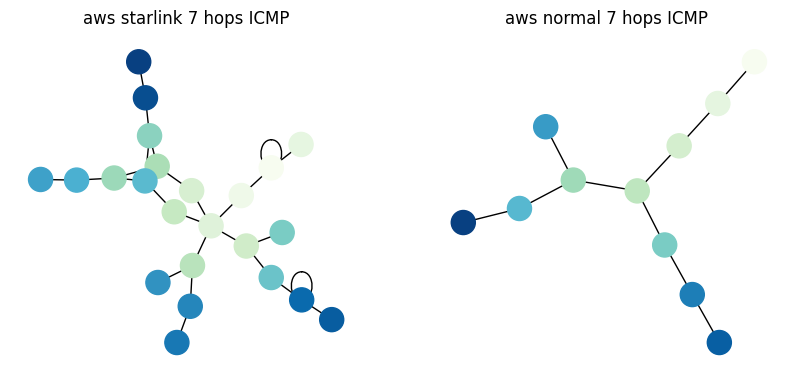
\includegraphics[width=0.75\textwidth]{pics/aws_7_icmp.png}
        % \caption{First seven hops of traceroutes to 5 AWS datacenters using ICMP; left is Starlink, right is cabled connection}
    \end{figure}
\end{frame}

\begin{frame}{Visualize Visible Satellites}
    Can we visualize visible satellites?
    \begin{itemize}
        \item Two-line element sets (TLE)\footnote{\url{https://en.wikipedia.org/wiki/Two-line_element_set}}: 
        \begin{itemize} 
            \item A data format encoding information about Earth-orbiting object for a given point in time
            \item Allow for estimation of position and velocity at any point in the past or future
        \end{itemize}     
        \item Downloaded a list of Starlink's satellites TLEs from \href{celestrak.org}{celestrak.org}
        \item Wrote a python script to calculate visible
        satellites\footnote{\url{https://gitlab.lrz.de/netintum/teaching/tumi8-theses/idp-castellotti/-/blob/main/common.py?ref_type=heads\#L132}}
        \item Gathered information about satellite position
        \item Visualized patterns in satellite appearances.
    \end{itemize}
\end{frame}

\begin{frame}{Visualizing Patterns in Visible Satellites}
    \begin{figure}
        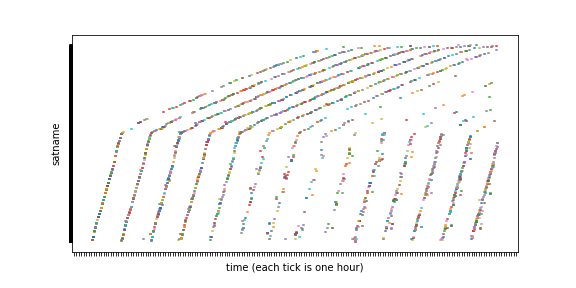
\includegraphics[width=0.9\textwidth]{pics/patterns-in-satellite-appearances.png}
        % \caption{Visualizing patterns in Visible Satellites, we add a dot whenever we see a satellite}
    \end{figure}
\end{frame}

\begin{frame}{Physical Layer Influences on Performance}
    Does the physical layer have any influences on performance? 
    \begin{itemize}
        \item We wanted to understand whether the physical layer influences RTT
        \item The Dish may decide to send a packet only when it fills a buffer
        \item Sent packets to a host we control with iPerf to create traffic on the interface, varying the payload size
        \item Downloaded Debian ISOs from 5 different mirrors (to neutralize upload speed differences)
        \item Measured RTTs 
    \end{itemize}
\end{frame}

\begin{frame}{{Physical Layer Influences on Performance}}
    \begin{figure}
        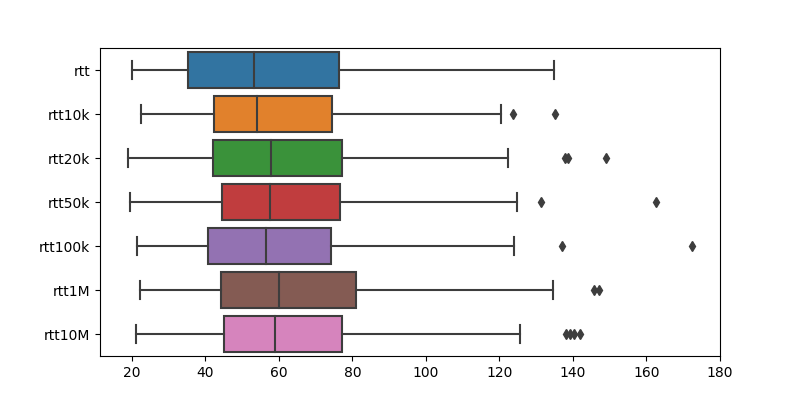
\includegraphics[width=0.8\textwidth]{pics/rtt-iperf-stress.png}
        \caption{Physical Layer Influences on Performance}
    \end{figure}
\end{frame}

\begin{frame}{The \texttt{dish\_get\_obstruction\_map} Endpoint}
    Can we use a side channel to extract satellite handovers from obstruction maps?
    \begin{itemize}
        \item An obstruction map captures the position where the Dish has seen satellites
        \item Designed to provide a way to report whether the dish positioning is optimal
        \item Following the approach described by Izhikevich et al. \cite{izhikevich2023democratizing}, we retrieved maps
        \begin{itemize}
            \item Reboot the Dish to clear the obstruction map (\texttt{api.reboot})
            \item Poll the endpoint frequently enough to see satellite traces (\texttt{api.get\_obstruction\_map})
            \item Save the maps to visualize them later
        \end{itemize}
    \end{itemize}
\end{frame}

\begin{frame}[fragile]{Querying the \texttt{dish\_get\_obstruction\_map} Endpoint }
    \begin{lstlisting}
"apiVersion":"9",
"dishGetObstructionMap":{
    "minElevationDeg":10.0,
    "numCols":123,
    "numRows":123,
    "snr":[-1.0,-1.0,-1.0,-1.0,...,1.0,1.0,-1.0,-1.0]
}
    \end{lstlisting}
    \begin{itemize}
        \item Interpret the \texttt{"snr"} field as a matrix, it contains 15129 (123*123) items
        \item Export this as images using Matplotlib, adding a timestamp for each map
    \end{itemize}
\end{frame}

\begin{frame}[fragile]
    \begin{figure}
        \includegraphics<1>[width=0.4\columnwidth]{pics/map1.png}
        \includegraphics<2>[width=0.4\columnwidth]{pics/map2.png}
        \includegraphics<3>[width=0.4\columnwidth]{pics/map3.png}
        \includegraphics<4>[width=0.4\columnwidth]{pics/map4.png}
    \end{figure}
\end{frame}

\begin{frame}{Detecting Handovers Algoritmically}
    \begin{itemize}
        \item Going through visualizations frame by frame is not feasible (1000s of frames)
        \item Following the map matrix interpretation, we assume:
        \begin{itemize}
            \item "1" means a satellite was detected in that position
            \item  "-1" means no satellite was detected in that position
        \end{itemize} 
        \item Iterate through matrices two by two and sum them
        \item Check if, in the sum matrix, a "0" entry is "near" a "2" entry (inside a 3*3 matrix)
            \begin{itemize}
                \item If it is "near" \emph{no handover was performed}
                \item If it is in complete different position \emph{an handover must have been performed}
            \end{itemize}
    \end{itemize}
    \only<2>{
        $$\begin{bmatrix}
            -1 & \color{red}1 &           -1 & -1           \\
            -1 &           -1 & \color{red}1 & -1           \\
            -1 &           -1 &           -1 & -1           \\
            -1 &           -1 &           -1 & -1           \\
            \end{bmatrix}
            +
            \begin{bmatrix}
            -1 & \color{red}1 &           -1 &           -1 \\
            -1 &           -1 & \color{red}1 &           -1 \\
            -1 &           -1 &           -1 & \color{red}1 \\
            -1 &           -1 &           -1 &           -1 \\
            \end{bmatrix}
            =
            \begin{bmatrix}
            -2 & 2            &  -2          &           -2 \\
            -2 & -2           &  2           &           -2 \\
            -2 & -2           & -2           & \color{red}0 \\
            -2 & -2           & -2           &           -2 \\
        \end{bmatrix}$$
    }
    \only<3>{
        $$\begin{bmatrix}
            -1 & -1 & \color{red}1 &           -1          \\
            -1 & -1 &           -1 & \color{red}1          \\
            -1 & -1 &           -1 &           -1          \\
            -1 & -1 &           -1 &           -1          \\
        \end{bmatrix}
        +
        \begin{bmatrix}
            -1 & -1 & \color{red}1 &           -1          \\
            -1 & -1 &           -1 & \color{red}1          \\
            -1 & -1 &           -1 &           -1          \\
            1 & -1 &            -1 &           -1          \\
        \end{bmatrix}
        =
        \begin{bmatrix}
            -2           & -2 & 2 &  -2                    \\
            -2           & -2 & -2 &  2                    \\
            -2           & -2 & -2 & -2                    \\
            \color{red}0 & -2 & -2 & -2                    \\
        \end{bmatrix}$$
    }
\end{frame}

\begin{frame}[fragile]{Correlating Satellite Handovers and Bandwidth Drops}
    Is there any correlation between satellite handovers and drops in bandwidth?
    \begin{itemize}
        \item We now have an algorithm to detect handovers
        \item We run two scripts in parallel:
            \begin{itemize}
                \item 1st: retrieves an obstruction map every second
                \item 2nd: gathers bandwidth data
            \end{itemize} 
        \item We visualize bandwidth data and satellite handovers 
    \end{itemize}
\end{frame}

\begin{frame}[fragile]{Correlating Satellite Handovers and Bandwidth Drops}
    \begin{figure}
        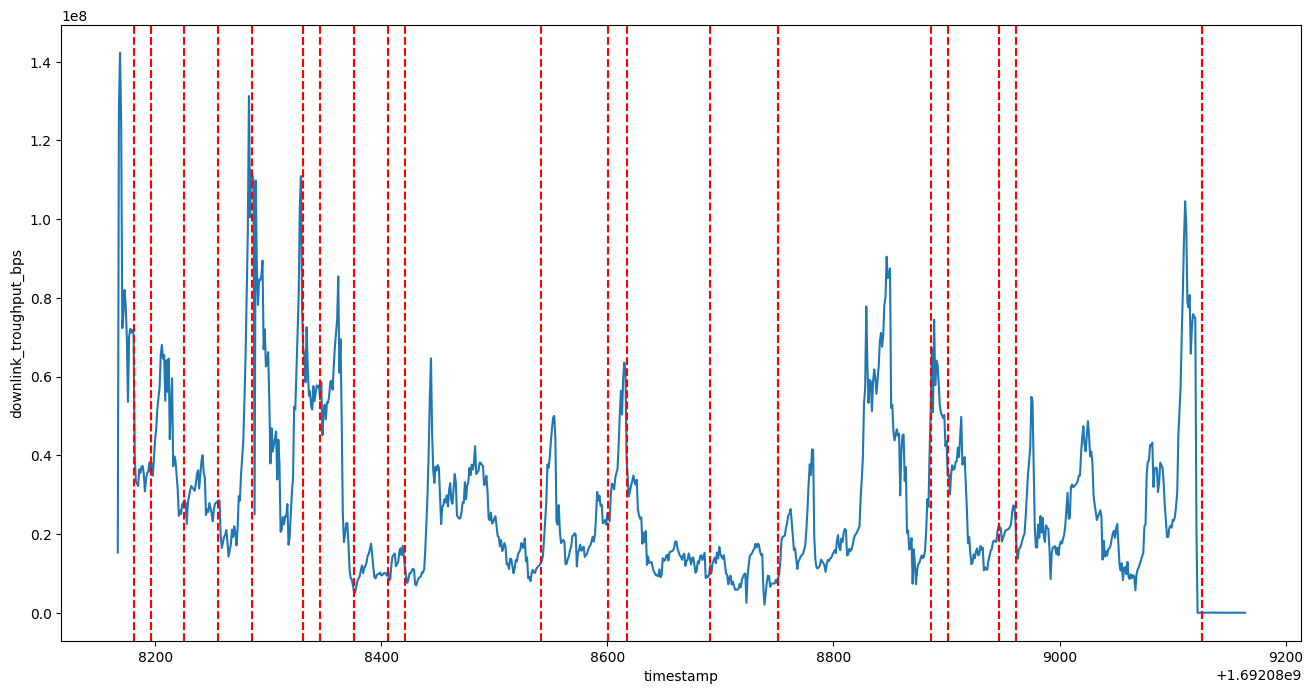
\includegraphics[width=0.8\columnwidth]{pics/correlation_handovers_bw.png}
        % \caption{Correlating Satellite Handovers and Bandwidth Drops, blue is bandwidth, red vertical dashes are satellite handovers}
    \end{figure}
\end{frame}

\begin{frame}[fragile]{Final Remarks}
    We conclude that:
    \begin{itemize}
        \item Majority of the Endpoints on the gRPC API are not accessible
        \item PoP Latency is remarkably stable
        \item Physical layer has no remarkable influences on performance
        \item Bandwidth is sustained consistently, even in the presence of satellite handovers
        \item Getting insights into inner routing is hard
    \end{itemize}
\end{frame}

\begin{frame}[fragile]{Future Work}
    Further research might include:
    \begin{itemize}
        \item Running the same measurements over a longer period of time
        \item Analyzing routing using IPv6
        \item Repeating the measurements with different satellite constellations
        \item Analyze ISL routing (first hop after AS14593)
    \end{itemize}
\end{frame}

\section{Bibliography}
\begin{frame}[allowframebreaks]
    \bibliographystyle{abbrv}
    \setbeamertemplate{bibliography item}[text]
    \footnotesize
    \bibliography{lit}
\end{frame}

\end{document}
